\documentclass[a4paper]{scrreprt}

% Uncomment to optimize for double-sided printing.
% \KOMAoptions{twoside}

% Set binding correction manually, if known.
% \KOMAoptions{BCOR=2cm}

% Localization options
\usepackage[english]{babel}
\usepackage[T1]{fontenc}
\usepackage[utf8]{inputenc}

% Sub figures
\usepackage{subcaption}

% Quotations
\usepackage{dirtytalk}

% Floats
\usepackage{float}

% Enhanced verbatim sections. We're mainly interested in
% \verbatiminput though.
\usepackage{verbatim}

% Automatically remove leading whitespace in lstlisting
\usepackage{lstautogobble}

% CSV to tables
\usepackage{csvsimple}

% PDF-compatible landscape mode.
% Makes PDF viewers show the page rotated by 90°.
\usepackage{pdflscape}

% Advanced tables
\usepackage{array}
\usepackage{tabularx}
\usepackage{longtable}

% Fancy tablerules
\usepackage{booktabs}

% Graphics
\usepackage{graphicx}

% Current time
\usepackage[useregional=numeric]{datetime2}

% Float barriers.
% Automatically add a FloatBarrier to each \section
\usepackage[section]{placeins}

% Custom header and footer
\usepackage{fancyhdr}

\usepackage{geometry}
\usepackage{layout}

% Math tools
\usepackage{mathtools}
% Math symbols
\usepackage{amsmath,amsfonts,amssymb}
\usepackage{amsthm}
% General symbols
\usepackage{stmaryrd}

% Utilities for quotations
\usepackage{csquotes}

% Bibliography
\usepackage[
  style=alphabetic,
  backend=biber, % Default backend, just listed for completness
  sorting=ynt % Sort by year, name, title
]{biblatex}
\addbibresource{references.bib}

\DeclarePairedDelimiter\abs{\lvert}{\rvert}
\DeclarePairedDelimiter\floor{\lfloor}{\rfloor}

% Bullet point
\newcommand{\tabitem}{~~\llap{\textbullet}~~}

\pagestyle{plain}
% \fancyhf{}
% \lhead{}
% \lfoot{}
% \rfoot{}
% 
% Source code & highlighting
\usepackage{listings}

% SI units
\usepackage[binary-units=true]{siunitx}
\DeclareSIUnit\cycles{cycles}

\newcommand{\lecture}{41109 - Privacy and Data Security}
\newcommand{\series}{11}
% Convenience commands
\newcommand{\mailsubject}{\lecture - Series \series}
\newcommand{\maillink}[1]{\href{mailto:#1?subject=\mailsubject}
                               {#1}}

% Should use this command wherever the print date is mentioned.
\newcommand{\printdate}{\today}

\subject{\lecture}
\title{Series \series}

\author{Michael Senn \maillink{michael.senn@students.unibe.ch} --- 16-126-880}

\date{\printdate}

% Needs to be the last command in the preamble, for one reason or
% another. 
\usepackage{hyperref}

\begin{document}
\maketitle


\setcounter{chapter}{\numexpr \series - 1 \relax}

\chapter{Series \series}

\section{Information-theoretic steganography}

Recall that an ideal covertext distrubtion $C$ can be split into two disjoint
subsets $\bar{C}$ and $\hat{C}$ such that their respective sums of
probabilities are as close as possible.

Using a brute-force algorithm to solve the partitioning problem yields that the
covertext distribution $C$ can be split into the most even subsets, namely:

\begin{align*}
		\hat{C} & \coloneqq \{a, b, d, e\} \\
		\bar{C} & \coloneqq \{c, f, g, h\}
\end{align*}

Then the difference in sums of probabilities is minimal:
\[
		\epsilon = \abs*{
				\sum_{c \in \hat{C}} P(\hat{C} = c) - 
		        \sum_{c \in \bar{C}} P(\bar{C} = c)} 
		= 0.04
\]

As such, this is an $\epsilon^2 / \log_e(2) \approx 0.0023$-statistically
secure stegosystem.

\section{Practical steganography}

Using `steghide', messages were embedded in a $448 \times 274$ bitmap image.
The largest message which could be emdedded was \SI{30}{\kilo\byte}.  Figure
\ref{fig:steganography} shows the cover image on the left, the image with the
embedded \SI{30}{\kilo\byte} text data on the right, and the difference of
the two images in the middle.  Clearly, no difference is visible to the naked
eye.

A comparison using a hexeditor shows that various bytes, spread throughout the
file, had their lower-order bits changed. One such difference is shown below.

\begin{lstlisting}
< 0001e040: 2b2b 2b2b 2b2b 2b2b 2b2b 2b2b 2b2b 2b2b
> 0001e040: 2b2b 312b 2b2b 2c2b 2b2b 292c 2b2c 2c2b
\end{lstlisting}

It should be noted that the cover image --- by virtue of being a
black-and-white digital drawing --- has very little variance. Indeed it consist
mainly of cleanly separated regions of uniform colour. The modified image
however, as its low-order bits were changed in multiple places, tends to have
noticeably more variance in certain regions. It is plausible that this would
allow to distinguish the stegotext and covertext distributions.

\begin{figure}
		\centering
		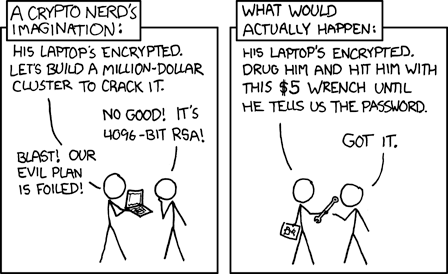
\includegraphics[width=0.7\linewidth]{resources/coverfile} \\
		
\includegraphics[width=0.7\linewidth]{resources/difference} \\
		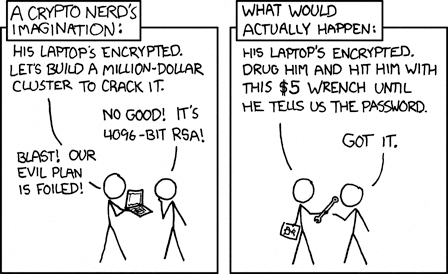
\includegraphics[width=0.7\linewidth]{resources/stegofile_30k}
		\caption{
				Effect of hiding \SI{30}{\kilo\byte} text inside comic using
				`steghide'. Original image on top, modified image on bottom, difference
				in the middle.
		}
		\label{fig:steganography}
\end{figure}

\printbibliography

\end{document}
